\documentclass[conference]{IEEEtran}
\usepackage{cite}
\usepackage{amsmath,amssymb}
\usepackage{graphicx}
\usepackage{booktabs}
\usepackage{url}
\usepackage[T1]{fontenc}
\usepackage{tikz}
\usetikzlibrary{arrows.meta,positioning,fit}
\usepackage{microtype}
\usepackage{xcolor}
\graphicspath{{assets/}}
\def\BibTeX{{\rm B\kern-.05em{\sc i\kern-.025em b}\kern-.08em T\kern-.1em\lower.7ex\hbox{E}\kern-.125em X}}

\begin{document}

\title{TrialMatch: Criterion-Level Clinical Trial Screening with a LoRA-Tuned Qwen2.5 Decoder and a From-Scratch KV-Cache, Tiled-Attention and Speculative-Decoding Engine}

\author{\IEEEauthorblockN{Muhammad Musa Khan}
\IEEEauthorblockA{Generative AI, Semester 7\\
Roll No.: 23i-0526\quad mmk240705@gmail.com}}

\maketitle

\begin{abstract}
We build an end-to-end, educational screening prototype that reads a patient description, one trial criterion (inclusion or exclusion), and returns a structured eligibility label together with the supporting patient-sentence IDs. A Qwen2.5-1.5B-Instruct decoder is adapted with LoRA on the prescribed patient-grouped split (37/8/8 patients) of the TrialGPT Criterion Annotations. Beyond fine-tuning, we implement the Transformer inference machinery ourselves: a hand-written Qwen2 forward pass with an explicit KV cache, a reference and a tiled online-softmax attention kernel, and greedy speculative decoding with a fine-tuned Qwen2.5-0.5B draft and cache rollback. Every mechanism is validated against a reference (token equality, numerical error against fp64) and benchmarked on a free Colab T4 GPU. The system is exposed through a browser application that screens a note against user-entered criteria, shows each decision with its evidence, compares decoding modes live, and exports a report. \emph{This is a research prototype, not a clinical enrolment tool.}
\end{abstract}

\begin{IEEEkeywords}
clinical trial matching, LoRA, KV cache, online softmax attention, speculative decoding, evidence retrieval
\end{IEEEkeywords}

\section{Introduction and Problem Statement}
Matching patients to clinical trials requires reading free-text notes against long lists of inclusion and exclusion criteria. TrialGPT~\cite{trialgpt} showed that large language models can judge each criterion, cite the sentences that justify it, and aggregate the judgements. Its strongest results rely on proprietary GPT-4. Our goal is narrower and fully open: given a patient note, a criterion type and a criterion text, an open-weight decoder that fits a free T4 GPU must return (i) one of the dataset's expert label categories, including \emph{not enough information} and \emph{not applicable}, and (ii) the IDs of the supporting sentences, so that every decision can be audited.

The assignment also requires understanding the machinery that makes such models usable: key/value caching, memory-efficient attention and speculative decoding. We therefore treat the system as two coupled problems: a \emph{task} problem (accurate, evidence-grounded criterion classification) and a \emph{systems} problem (fast, verifiably correct autoregressive inference). Our contributions are: (1) a LoRA-adapted Qwen2.5-1.5B criterion classifier evaluated on the fixed held-out split before/after tuning; (2) a hand-written decoder with an explicit KV cache verified token-for-token against a no-cache reference and the Hugging Face implementation; (3) a tiled online-softmax attention implementation validated against fp64; (4) greedy speculative decoding with cache rollback and a task-tuned draft; (5) a browser application exposing all of the above.

\section{Related Work}
\textbf{Clinical trial matching.} TrialGPT~\cite{trialgpt} decomposes matching into criterion-level classification with sentence-level evidence, then ranks trials; the released criterion annotations are our only training and evaluation data. We reuse its label vocabulary but never use the GPT-4 predictions or explanations contained in the data as input or features.

\textbf{Open-weight decoders and adaptation.} Qwen2.5~\cite{qwen25} offers Apache-2.0 decoder models from 0.5B to 72B parameters with grouped-query attention (GQA)~\cite{gqa} and rotary position embeddings (RoPE)~\cite{rope}, and a 0.5B member that shares the 1.5B tokenizer, which matters for speculative decoding. LoRA~\cite{lora} adapts a frozen model by learning low-rank updates to linear layers, and QLoRA~\cite{qlora} adds 4-bit quantisation; with a 1.5B model on a 15\,GB GPU, half-precision LoRA suffices and avoids quantisation noise.

\textbf{Efficient attention.} The Transformer~\cite{transformer} attention matrix is quadratic in sequence length. Online (streaming) softmax~\cite{online} computes the normaliser in one pass, and FlashAttention~\cite{flash} combines it with tiling so the score matrix is never materialised, reducing memory traffic. We implement the tiling and online-softmax recurrence ourselves in PyTorch and compare it with PyTorch's fused scaled-dot-product attention.

\textbf{Inference acceleration.} Caching keys and values removes the recomputation of earlier tokens during decoding~\cite{pope}. Speculative decoding~\cite{specdec,specsamp} lets a small draft model propose several tokens that the target verifies in one forward pass; with greedy decoding the output is identical to the target's own greedy output, and the speedup depends on the draft's acceptance rate and relative cost.

\textbf{Alternatives and why we did not use them.} There are several other techniques we could have used, but each comes with certain limitations for this project. GPT-4-based matching~\cite{trialgpt} provides very high accuracy, but it relies on a paid and closed API, which is not allowed by the assignment. It also does not give us access to the internal workings that we are required to study. Full fine-tuning is another option, but it updates all the model weights and requires additional memory for storing optimiser states. For a 1.5B model, this exceeds what we can comfortably run on a 15\,GB GPU. QLoRA~\cite{qlora} could allow us to work with larger models, but it introduces quantisation noise and additional de-quantisation overhead, which we do not really need for a model of this size.

Similarly, PagedAttention~\cite{vllm} is mainly useful for managing the KV cache efficiently when serving multiple concurrent requests. Since our setup uses a batch size of one and context lengths below 2,500 tokens, a simple pre-allocated contiguous cache is sufficient. We also considered draft-free acceleration methods such as Medusa~\cite{medusa} and EAGLE~\cite{eagle}. These methods add extra decoding heads to the target model, avoiding the need for a second model. However, they require additional training and make it harder to compare the results against a standard greedy decoding baseline. Therefore, we decided to use the conventional two-model draft/target approach.

Finally, FlashAttention~\cite{flash} is implemented as a fused CUDA kernel. However, our assignment focuses on understanding and implementing the algorithm itself rather than using a particular optimised kernel. So, we implement the tiling strategy and online-softmax recurrence directly in PyTorch, while using PyTorch's SDPA as our optimised reference for comparison.

\section{Materials and Methods}
\subsection{Dataset and Patient-Grouped Split}
We use only \texttt{ncbi/TrialGPT-Criterion-Annotations}: 1,015 criterion-level annotations from 53 patients. Each record has a numbered patient note, trial title, criterion type and text, an expert eligibility label, and expert sentence IDs. Fields produced by GPT-4 (\texttt{gpt4\_explanation}, \texttt{explanation\_correctness}, \texttt{gpt4\_sentences}, \texttt{gpt4\_eligibility}) and the dataset's own \texttt{training} flag are dropped before any model sees the data. Following the protocol, the 53 sorted unique patient IDs are permuted with NumPy \texttt{default\_rng(42)} and assigned 37/8/8 patients to train/validation/test; every annotation of a patient stays in one split. This yields 603/206/206 annotations. A script asserts that the patient sets are disjoint and the manifest (patient IDs and counts) is published. The test split was used for the final evaluation only, after all choices were fixed on validation.

\subsection{Candidate Models and Selection}
We considered open-weight decoders that could be fine-tuned and served on a 15\,GB T4 (Table~\ref{tab:models}; parameters and shapes read from the model configurations). Qwen2.5-3B was rejected because fp16 weights (5.7\,GB) plus LoRA activations leave little headroom, its licence is non-commercial research only, and it would double decode cost. SmolLM2-1.7B uses full multi-head attention (32 KV heads), so its KV cache is $6.9\times$ larger per token than Qwen2.5-1.5B, and its 49k vocabulary and 8k context are less convenient. TinyLlama-1.1B has a 2k context and a different tokenizer, so none of the available small drafts would be compatible. We selected \textbf{Qwen2.5-1.5B-Instruct}: Apache-2.0, 1.54B parameters (3.1\,GB in fp16), 28 layers, 12 query / 2 KV heads (GQA), head dimension 128, 32k context, 151,936-token vocabulary, only 28\,KiB of KV cache per token, and a same-tokenizer 0.5B sibling (Qwen2.5-0.5B-Instruct; 24 layers, 14/2 heads, head dimension 64) for the draft. Training notes are short (at most 581 tokens including the answer), so truncation is not a concern.

\begin{table}[t]
\caption{Candidate decoders (from model configs). KV B/tok = fp16 cache bytes per token.}
\label{tab:models}
\centering\scriptsize
\resizebox{\columnwidth}{!}{\begin{tabular}{lccccccc}\toprule Model & Params & Layers & Q/KV heads & Ctx & fp16 GB & KV B/tok & License\\\midrule
Qwen2.5-1.5B & 1.54B & 28 & 12/2 & 32k & 2.9 & 28,672 & Apache-2.0\\
Qwen2.5-0.5B & 0.49B & 24 & 14/2 & 32k & 0.9 & 12,288 & Apache-2.0\\
Qwen2.5-3B & 3.09B & 36 & 16/2 & 32k & 5.7 & 36,864 & Qwen-research\\
SmolLM2-1.7B & 1.71B & 24 & 32/32 & 8k & 3.2 & 196,608 & Apache-2.0\\
TinyLlama-1.1B & 1.10B & 22 & 32/4 & 2k & 2.0 & 22,528 & Apache-2.0\\
\bottomrule\end{tabular}}
\end{table}

\subsection{Input/Output Schema and Fine-Tuning}
The prompt is the Qwen chat template with a fixed system instruction, the numbered patient note, the criterion type and the criterion text. The target is a JSON object followed by the end-of-turn token, e.g.\ \texttt{\{"label": "included", "evidence": [0]\}}. Labels come from the dataset (inclusion: \emph{included, not included, not enough information, not applicable}; exclusion: \emph{excluded, not excluded, not enough information, not applicable}); evidence is the list of expert sentence IDs. The loss is the cross entropy over the completion tokens only (prompt tokens are masked), normalised by the number of target tokens in each optimiser step.

We fine-tune with LoRA (rank 16, $\alpha{=}32$, dropout 0.05) on all seven attention and MLP projections, giving 18.5M trainable parameters (1.2\% of the model); the base weights stay in fp16, adapters are fp32, and we use fp16 autocast with a gradient scaler and gradient checkpointing. Optimiser: AdamW, peak learning rate $2\times10^{-4}$, 5 warm-up steps then cosine decay, gradient clipping at 1.0, micro-batch 2 with 8 accumulation steps (effective batch 16), 4 epochs (152 optimiser steps), seed 42. Because the labels are imbalanced (Table~\ref{tab:dist}), mini-batches are drawn with replacement with weights proportional to $n_c^{-p}$, where $n_c$ is the training count of the example's label; the first run uses $p{=}0.5$ (v1) and an alternative uses $p{=}1$ (v2). The epoch with the best validation macro-F1 is kept. The 0.5B draft is tuned with the identical recipe (micro-batch 4, accumulation 4).

\begin{table}[t]
\caption{Annotations per split (patients in parentheses) and label distribution (criterion type: label).}
\label{tab:dist}
\centering\scriptsize
\resizebox{\columnwidth}{!}{\begin{tabular}{llrrr}\toprule Type & Label & Train & Val & Test\\\midrule
\multicolumn{2}{l}{Annotations (patients)} & 603 (37) & 206 (8) & 206 (8)\\
inclusion & included & 88 & 35 & 27\\
inclusion & not included & 13 & 3 & 7\\
inclusion & not enough info. & 109 & 27 & 38\\
inclusion & not applicable & 5 & 1 & 3\\
exclusion & excluded & 8 & 2 & 0\\
exclusion & not excluded & 292 & 101 & 91\\
exclusion & not enough info. & 65 & 26 & 28\\
exclusion & not applicable & 23 & 11 & 12\\
\bottomrule\end{tabular}}
\end{table}

\subsection{Evaluation Protocol}
Predictions are parsed from the generated JSON; an output whose label is not valid for the criterion type is counted as wrong (\textsc{invalid}). We report accuracy and macro-F1 over the gold classes, per-class precision/recall/F1 and confusion matrices, overall and separately for inclusion and exclusion. Evidence is scored per criterion on sets of sentence IDs: micro precision/recall/F1 pool all sentences; macro-F1 averages the per-criterion F1, where two empty sets score 1 and one empty set scores 0. In this data every annotation has at least one gold sentence, so an empty prediction is always a miss. Absence of evidence is never converted to a label by the system.

\subsection{Engine: Hand-Written Qwen2 Forward Pass with KV Cache}
To avoid relying on \texttt{use\_cache=True}, we implement the Qwen2 decoder forward pass ourselves, reusing only the weights (LoRA merged into the base matrices). Each layer applies RMSNorm, the q/k/v projections (with bias), RoPE, grouped-query attention, the output projection, a second RMSNorm and the SwiGLU MLP, with residual connections.

\emph{Positional handling.} For a block of $T$ new tokens and a cache holding $n$ tokens, token $i$ gets absolute position $n+i$; RoPE is applied to the new queries and keys with these positions \emph{before} the keys are cached, so cached keys never need re-rotation.

\emph{Cache update and growth.} The cache is a pre-allocated tensor of shape $[B,H_{kv},T_{max},d]$ per layer for keys and values. A step writes the new $K,V$ at positions $[n,n+T)$ and attention runs over the valid prefix $[0,n+T)$. Memory grows linearly: $2\cdot L\cdot H_{kv}\cdot d\cdot b = 28{,}672$ bytes per token for the 1.5B model ($L{=}28$, $H_{kv}{=}2$, $d{=}128$, $b{=}2$), i.e.\ 28\,MiB per 1,024 tokens; GQA makes this $6\times$ smaller than full multi-head attention.

\emph{Masking.} A query at block offset $i$ sits at absolute position $n+i$ and may attend to keys $j\le n+i$, i.e.\ a lower-triangular mask with diagonal offset $T_k-T_q$. Single-token decoding needs no mask; multi-token blocks (prefill and speculative verification) use the offset mask.

\emph{Paths.} The \textbf{reference} path rebuilds an empty cache and re-runs the whole sequence for every generated token. The \textbf{cached} path prefils once and then feeds one token per step. Both use the same kernels, so differences isolate cache reuse. Decoding is greedy (argmax) with the end-of-turn token as stop.

\subsection{Reference and Tiled Online-Softmax Attention}
The reference computes $S=QK^\top/\sqrt d$, applies the causal mask, subtracts the row maximum, exponentiates and normalises, all in fp32. The tiled variant processes query blocks of size $B_q$ and streams key/value blocks of size $B_k$, keeping for each query row a running maximum $m$, normaliser $\ell$ and unnormalised output $O$:
\begin{align}
m' &= \max\!\big(m,\ \mathrm{rowmax}(S_j)\big), \quad P = e^{S_j-m'},\\
\ell &\leftarrow e^{m-m'}\ell + \mathrm{rowsum}(P),\
O &\leftarrow e^{m-m'}O + P V_j,\quad m \leftarrow m',
\end{align}
and outputs $O/\ell$ after the last block. Key blocks that lie entirely in the future of every query in the block are skipped. Only a $B_q\times B_k$ score tile exists at any time. In pure PyTorch each tile is a separate kernel launch, so we expect the tiled version to save memory but not time compared with fused kernels; we measure this in Section~\ref{sec:attn}. The model can run with either kernel, and we check end-to-end token equality for the tiled one.

\subsection{Greedy Speculative Decoding}
A fine-tuned Qwen2.5-0.5B (same tokenizer) drafts $K$ tokens; the 1.5B target verifies them in one forward pass. In each round, with $x_0$ the last emitted token (not yet in the target cache) and drafts $d_1..d_K$, the target processes $[x_0,d_1,\dots,d_K]$ and returns predictions $p_0..p_K$ ($p_i$ follows the $i$-th input). The accepted length is $n=\max\{i:\ d_{j}=p_{j-1}\ \forall j\le i\}$; the round emits $d_1..d_n$ and $p_n$ (a correction, or a bonus token when $n{=}K$). The target cache is rolled back to the accepted prefix by moving its length pointer; the draft cache is rolled back the same way, except when $n{=}K$ the draft never processed $d_K$ and receives it with the next block. With greedy decoding the emitted tokens equal those of target-only greedy decoding. If the per-token acceptance is $\alpha$, one round yields $(1-\alpha^{K+1})/(1-\alpha)$ tokens in expectation, at the cost of $K$ draft steps and one $(K{+}1)$-token target pass.

\subsection{Application Workflow}
Fig.~\ref{fig:sys} shows the system. A user pastes a note (sentences are numbered automatically in the training format), adds criteria and selects a decoder (no cache, KV cache or speculative). For each criterion the engine returns the label and sentence IDs; the application resolves the IDs to the original sentence text, flags cited IDs that do not exist or definitive labels without evidence (\emph{unsupported}), and builds an explanation \emph{only} from the cited sentences. An explicit, transparent rule set (R1--R4 in the application's ``About'' tab) aggregates criterion labels into a preliminary patient-trial outcome; this aggregation is not ground truth. The page also provides a live comparison of the three decoders (time, tokens/s, peak GPU memory, token equality), an attention lab, saved experiment tables, and a downloadable HTML/JSON report with provenance and a disclaimer that this is an educational screening prototype.

\begin{figure}[t]
\centering
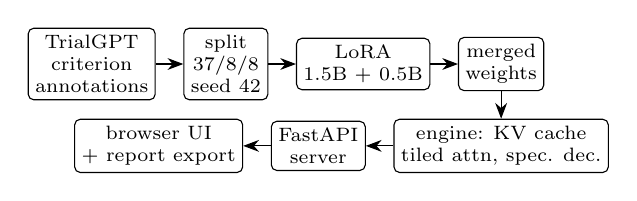
\begin{tikzpicture}[node distance=3.5mm, every node/.style={font=\scriptsize}, box/.style={draw,rounded corners=2pt,align=center,minimum height=6mm,inner sep=2.5pt}, >={Stealth[length=2mm]}]
\node[box] (d) {TrialGPT\\criterion\\annotations};
\node[box,right=of d] (s) {split\\37/8/8\\seed 42};
\node[box,right=of s] (l) {LoRA\\1.5B + 0.5B};
\node[box,right=of l] (m) {merged\\weights};
\node[box,below=of m] (e) {engine: KV cache\\tiled attn, spec. dec.};
\node[box,left=of e] (a) {FastAPI\\server};
\node[box,left=of a] (u) {browser UI\\+ report export};
\draw[->] (d)--(s); \draw[->] (s)--(l); \draw[->] (l)--(m); \draw[->] (m)--(e); \draw[->] (e)--(a); \draw[->] (a)--(u);
\end{tikzpicture}
\caption{System overview: data preparation and adaptation (top) feed the inference engine behind the browser application (bottom).}
\label{fig:sys}
\end{figure}

\section{Experimental Setup}
All experiments ran on a free Google Colab session with one NVIDIA Tesla T4 (15\,GB), PyTorch with CUDA, Hugging Face Transformers/PEFT, and fp16 weights. Training used the recipe above; decoding benchmarks used a single prompt (batch size 1), one warm-up run, 3 timed repetitions (2 for the no-cache path), CUDA synchronisation around every timing, and peak extra memory measured with \texttt{torch.cuda.max\_memory\_allocated} above the resident weights. Input lengths are formed by concatenating real test prompts and outputs are forced to a fixed length (no early stop) for the cache experiments. The speculative experiments use real test prompts with the natural stop token. The test split was evaluated exactly once with the final adapter chosen on validation data.

\section{Results and Discussion}

\subsection{Model Selection and Fine-Tuning (Tasks 1 and 2)}
\textbf{Training behaviour.} Fig.~\ref{fig:train} (left) shows the completion-token loss falling from about 0.2 to below 0.03 within the 152 optimiser steps; the right panel shows validation scores per epoch. For the selected run (v1) validation macro-F1 peaked at epoch~1 (0.481) and then drifted down to 0.436, while accuracy peaked at epoch~2 (0.748) and evidence F1 kept improving until epoch~4 (0.610). With only 8 validation patients and a handful of rare-class examples, macro-F1 moves by several points between epochs, so this selection is noisy. We nevertheless kept the pre-declared rule (best validation macro-F1), which selects epoch~1. The alternative v2, with fully inverse-frequency sampling ($p{=}1$), under-trained the majority classes: its best validation macro-F1 was 0.395 and its first-epoch accuracy only 0.437 with four unparsable outputs, so it was rejected. The 0.5B draft, trained with the same recipe, reached validation macro-F1 0.540 (epoch~3), which we kept for speculative decoding.

\begin{figure*}[t]
\centering
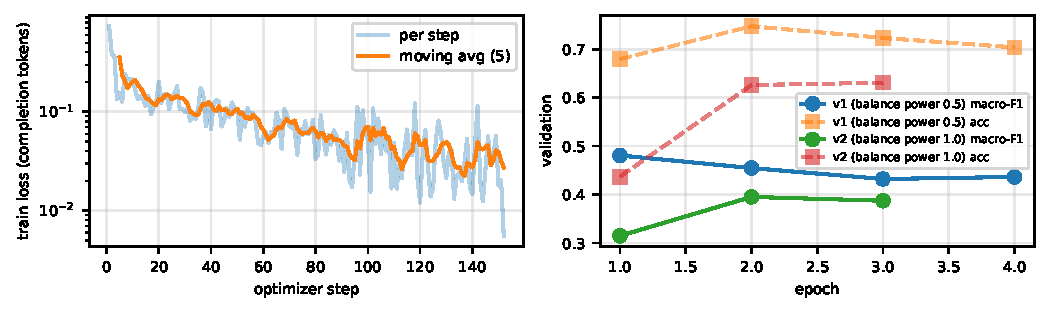
\includegraphics[width=\textwidth]{fig_train.pdf}
\caption{Training loss of the selected 1.5B run (left) and validation macro-F1 / accuracy per epoch for v1 and v2 (right).}
\label{fig:train}
\end{figure*}

\textbf{Before vs.\ after fine-tuning.} On the validation split the base model scores accuracy 0.087, macro-F1 0.095 and evidence F1 0.126 against 0.680/0.481/0.496 after tuning (epoch~1). Table~\ref{tab:main} gives the held-out test results, evaluated once. The zero-shot model rarely follows the required JSON schema (7 invalid outputs) and reaches an accuracy of 0.121; the adapted model reaches 0.723, macro-F1 0.685 and evidence micro-F1 0.559 with no invalid output. The two trivial baselines show what a model must beat: always predicting the training-majority label per criterion type already gives 0.626 accuracy (because 62.6\% of test criteria carry the majority label of their type) but only 0.272 macro-F1, and citing sentence~0 gives evidence F1 0.253. Hence the gain over the majority baseline is modest in accuracy (+0.097) but large in macro-F1 (+0.41) and evidence F1 (+0.31). We did not compute significance tests; with 206 criteria from 8 patients, differences of a few points should not be over-interpreted.

\begin{table}[t]
\caption{Held-out test results (206 criteria, 8 patients), before/after tuning and baselines. Generation: Hugging Face \texttt{generate}, fp16, batch 16, greedy with the model's default repetition penalty of 1.1 (see text).}
\label{tab:main}
\centering\scriptsize
\begin{tabular}{lcccc}\toprule System & Acc & Macro-F1 & Evid. $\mu$-F1 & Invalid\\\midrule
Majority label per type + sentence 0 & 0.626 & 0.272 & 0.253 & 0\\
Qwen2.5-1.5B zero-shot (before) & 0.121 & 0.172 & 0.167 & 7\\
Qwen2.5-1.5B + LoRA (after) & 0.723 & 0.685 & 0.559 & 0\\
\bottomrule\end{tabular}
\end{table}

\textbf{Decoding settings matter.} Qwen's bundled generation configuration sets a repetition penalty of 1.1 that Hugging Face applies even when sampling is disabled. Table~\ref{tab:main} was produced with this default, exactly as in the training-time validation. Our own engine implements plain greedy decoding (no penalty). Re-scoring the same held-out set with our engine (fp16, batch size 1, KV cache, argmax) gives accuracy 0.728, macro-F1 0.708 and evidence micro-F1 0.531 (inclusion 0.853/0.633/0.588; exclusion 0.656/0.484/0.410). Pure greedy is slightly better on accuracy and macro-F1 and worse on evidence F1; we regard the two runs as equivalent within noise and use the engine's decoding in the application.

\textbf{Inclusion vs.\ exclusion and per-class behaviour.} Table~\ref{tab:split} separates the two criterion types and Table~\ref{tab:perclass} lists per-class scores of the Table~\ref{tab:main} model. Inclusion is clearly easier (accuracy 0.840, evidence F1 0.66) than exclusion (0.656, 0.32). The test split contains no \emph{excluded} example (Table~\ref{tab:dist}), so macro-F1 is computed over the five classes that occur. For inclusion, \emph{included} (F1 0.87) and \emph{not enough information} (0.88) are handled well, \emph{not included} reaches F1 0.67 on only 7 examples, and \emph{not applicable} is never found (0 of 3). For exclusion, \emph{not excluded} (F1 0.79) dominates; \emph{not enough information} has recall 0.11 (3 of 28), i.e.\ the model usually asserts that an exclusion criterion does not apply when the note is merely silent, which is precisely the failure mode the task warns about. Fig.~\ref{fig:conf} shows the confusion matrices.

\begin{table}[t]
\caption{Test results separated by criterion type, with evidence precision/recall/F1 (micro).}
\label{tab:split}
\centering\scriptsize
\begin{tabular}{llcccc}\toprule System & Subset & Acc & Macro-F1 & Evid. P/R/F1 & n\\\midrule
Qwen2.5-1.5B zero-shot (before) & inclusion & 0.227 & 0.197 & 0.31/0.45/0.37 & 75\\
Qwen2.5-1.5B zero-shot (before) & exclusion & 0.061 & 0.077 & 0.03/0.25/0.06 & 131\\
Qwen2.5-1.5B + LoRA (after) & inclusion & 0.840 & 0.603 & 0.63/0.69/0.66 & 75\\
Qwen2.5-1.5B + LoRA (after) & exclusion & 0.656 & 0.484 & 0.38/0.28/0.32 & 131\\
\bottomrule\end{tabular}
\end{table}

\begin{table}[t]
\caption{Per-class precision, recall and F1 on the test set for the model of Table~\ref{tab:main}.}
\label{tab:perclass}
\centering\scriptsize
\begin{tabular}{llcccc}\toprule Subset & Class & P & R & F1 & Support\\\midrule
inclusion & included & 0.885 & 0.852 & 0.868 & 27\\
inclusion & not applicable & 0.000 & 0.000 & 0.000 & 3\\
inclusion & not enough information & 0.818 & 0.947 & 0.878 & 38\\
inclusion & not included & 0.800 & 0.571 & 0.667 & 7\\
exclusion & not applicable & 0.467 & 0.583 & 0.519 & 12\\
exclusion & not enough information & 0.231 & 0.107 & 0.146 & 28\\
exclusion & not excluded & 0.745 & 0.835 & 0.788 & 91\\
\bottomrule\end{tabular}
\end{table}

\begin{figure*}[t]
\centering
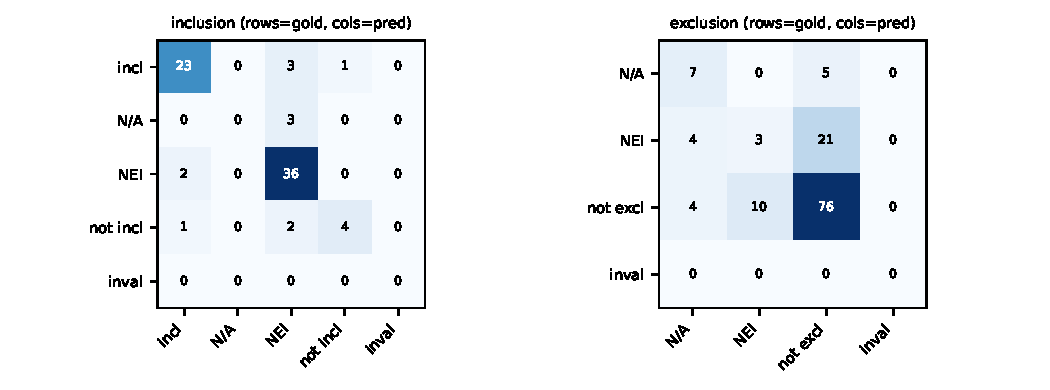
\includegraphics[width=0.85\textwidth]{fig_conf.pdf}
\caption{Test confusion matrices for inclusion and exclusion criteria (NEI = not enough information).}
\label{fig:conf}
\end{figure*}

\subsection{Error Analysis}
The model makes 57 label errors on the 206 test criteria. Table~\ref{tab:errors} lists twelve of them, one per distinct error type. We discuss them with the caveat that we did not trace internal causes; the explanations are hypotheses consistent with the outputs.
\begin{itemize}
\item \emph{Missing information treated as absence (cases 2, 5, 11).} For ``previous axillary surgery'' the gold label is \emph{not enough information} but the model answers \emph{not excluded} without citing any sentence; the application flags such answers as \emph{unsupported}. In case 11 the vague criterion ``Genetic patients'' is labelled \emph{included} with sentence~0 as evidence although the experts found the note uninformative.
\item \emph{Contradictory or hallucinated evidence (1, 7).} In case 1 the model cites sentence~1 to claim an exclusion that the experts judge not met; in case 7 it cites sentence~0 to support \emph{included} where the gold evidence set is empty. Both are fluent but wrong justifications.
\item \emph{Applicability confusion (4, 5, 6, 12).} The model predicts \emph{not applicable} for contraception-related exclusions that experts mark \emph{not excluded} or \emph{not enough information}, and the reverse in cases 6 and 12. Our reading is that \emph{not applicable} depends on patient characteristics (e.g.\ sex) that are expressed only indirectly in the note.
\item \emph{Negated criteria (8).} For ``No medical history of central vena catheterization'' the gold label is \emph{included} but the model says \emph{not included}, a typical negation inversion.
\item \emph{Missed or partial evidence (3, 10).} In case 3 the label is wrong though the right sentence is cited, and in case 10 the model cites sentence~0 whereas the experts used sentences 2 and 3, leading to \emph{not enough information} instead of \emph{included}.
\item \emph{Silent under-prediction (9).} For ``Maintenance hemodialysis after central vena catheterization'' the model predicts \emph{not enough information} and cites nothing, while the experts mark \emph{not included}.
\end{itemize}
Overall, errors cluster around information that is absent or implicit, which suggests that more annotated data or retrieval of related criteria would help more than additional epochs.

\begin{table*}[t]
\caption{Representative test errors, one per distinct error type (NEI = not enough information; ev. = evidence sentence IDs).}
\label{tab:errors}
\centering\scriptsize
\begin{tabular}{p{0.4cm}p{6.5cm}p{2.3cm}p{2.3cm}p{1.4cm}p{1.4cm}}\toprule \# & Criterion (truncated) & Gold & Pred & Gold ev. & Pred ev.\\\midrule
1 & Significant upper limb peripheral arterial disease & not excluded & excluded & [] & [1]\\
2 & Patients with previous axillary surgery & NEI & not excluded & [] & []\\
3 & Less than 18 years of age & not excluded & NEI & [0] & [0]\\
4 & Pregnant women or women of childbearing age who do not have adequate c... & not excluded & not applicable & [0] & []\\
5 & Female subject of child-bearing potential who is not using a medically... & NEI & not applicable & [] & [0]\\
6 & Symptoms that collectively suggest nonstreptococcal T/P (eg, laryngiti... & not applicable & not excluded & [0] & [0]\\
7 & Patients undergoing surgical lower limb revascularisation (suprainguin... & not included & included & [] & [0]\\
8 & No medical history of central vena catheterization. & included & not included & [0] & [0]\\
9 & Maintenance hemodialysis after central vena catheterization. & not included & NEI & [] & []\\
10 & Patients were included if they were diagnosed with Shock, Acute respir... & included & NEI & [2, 3] & [0]\\
11 & Genetic patients & NEI & included & [] & [0]\\
12 & If female, using birth control & not applicable & NEI & [3] & [3]\\
\bottomrule\end{tabular}
\end{table*}

\subsection{KV-Cached Generation (Task 3)}\label{sec:kv}
\textbf{Correctness.} Table~\ref{tab:equiv} compares our cached decoder with the no-cache reference and with Hugging Face \texttt{generate} for nine input/output length combinations (input prompts built from real test prompts, 128/512/1024 tokens; 16/64/128 forced output tokens, no early stopping). Cached and no-cache outputs are identical in all nine cases. Against \texttt{generate} with its default configuration six of nine differ, at positions 11--63; with the repetition penalty set to 1.0 all nine are identical, which shows that the discrepancy comes from the penalty and not from our implementation. In addition, on all 206 real test prompts our engine reproduces plain-greedy \texttt{generate} outputs exactly (206/206). In fp32 our forward pass matches Hugging Face to a maximum logit difference of $8.5\times10^{-5}$ with identical argmax at every position; in fp16 the corresponding difference on the same prompt is 0.088 and not all argmaxes agree, which is the expected size of half-precision rounding noise.

\begin{table}[t]
\caption{Cached decoding versus references (fp16, greedy). ``HF default'' includes Qwen's repetition penalty 1.1; ``HF pure'' sets it to 1.0.}
\label{tab:equiv}
\centering\scriptsize
\begin{tabular}{rrccc}\toprule In & Out & = no-cache & = HF default & = HF pure\\\midrule
128 & 16 & yes & yes & yes\\
128 & 64 & yes & no (@24) & yes\\
128 & 128 & yes & no (@24) & yes\\
512 & 16 & yes & no (@11) & yes\\
512 & 64 & yes & no (@11) & yes\\
512 & 128 & yes & no (@11) & yes\\
1024 & 16 & yes & yes & yes\\
1024 & 64 & yes & no (@63) & yes\\
1024 & 128 & yes & no (@63) & yes\\
\bottomrule\end{tabular}
\end{table}

\textbf{Performance.} Table~\ref{tab:cache} and Fig.~\ref{fig:cache} report the timings (batch 1, one warm-up, median of repeated runs with CUDA synchronisation). Without the cache the cost grows with the prompt length because every step recomputes the whole sequence, so the speedup rises from $1.3\times$ at 128 input tokens to $9.0\times$ at 2,048. With the cache, decoding runs at a nearly constant 27--29 tokens/s (about 35\,ms per token) regardless of context length, and prefill grows from 36\,ms to 378\,ms. The constant decode rate is far below what the T4's memory bandwidth would allow for 3\,GB of weights; it reflects Python and kernel-launch overhead of 28 layers executed eagerly, which is also why short prompts gain little. Peak additional memory is similar for both paths (e.g.\ 236 vs.\ 237\,MB at 2,048 tokens) because the cache is small---28\,KiB per token, about 56\,MiB for 2,048 tokens---and activations dominate; the no-cache path only pays in time.

\begin{table*}[t]
\caption{KV-cache benchmark: total time, speedup, prefill time, cached decode throughput, and peak extra memory (no-cache / cached).}
\label{tab:cache}
\centering\scriptsize
\begin{tabular}{rrrrrrrr}\toprule In & Out & No-cache s & Cached s & Speedup & Prefill s & Decode tok/s & Peak MB nc/c\\\midrule
128 & 32 & 1.41 & 1.09 & 1.3$\times$ & 0.036 & 29.4 & 16/13\\
128 & 128 & 6.00 & 4.43 & 1.4$\times$ & 0.036 & 28.9 & 24/16\\
512 & 32 & 3.85 & 1.16 & 3.3$\times$ & 0.080 & 28.7 & 51/50\\
512 & 128 & 16.19 & 4.71 & 3.4$\times$ & 0.081 & 27.4 & 61/52\\
1024 & 32 & 6.80 & 1.27 & 5.4$\times$ & 0.177 & 28.5 & 99/99\\
1024 & 128 & 28.10 & 4.72 & 6.0$\times$ & 0.181 & 28.0 & 108/101\\
2048 & 32 & 13.09 & 1.46 & 9.0$\times$ & 0.378 & 28.7 & 237/236\\
\bottomrule\end{tabular}
\end{table*}

\begin{figure}[t]
\centering
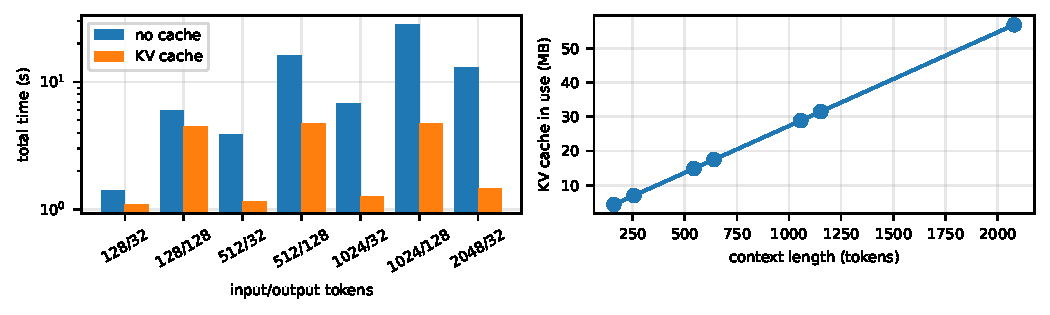
\includegraphics[width=\columnwidth]{fig_cache.pdf}
\caption{Left: total generation time with and without the KV cache. Right: KV cache bytes in use versus context length.}
\label{fig:cache}
\end{figure}

\subsection{Tiled Attention with Online Softmax (Task 4)}\label{sec:attn}
We tested 64 cases (8 shapes with batch 1--2, 4--14 heads, $T_q\in\{1,5,16,33,100,128,257,512\}$ and $T_k\ge T_q$, causal and non-causal, query scales 1 and 8 to stress the softmax, fp32 and fp16; tile sizes 32 and 128) against an fp64 reference. Table~\ref{tab:attnnum} shows that in fp32 the maximum absolute error of the tiled kernel ($1.6\times10^{-5}$) is comparable to that of the dense reference ($1.5\times10^{-5}$) and of PyTorch's SDPA ($1.4\times10^{-5}$), and that the tiled output differs from the dense reference by at most $8.4\times10^{-6}$; in fp16 all implementations are dominated by output rounding ($1.9\times10^{-3}$). The tiled kernel also drives the full model: greedy generation with it is token-identical to the SDPA path on the four prompts tested (24 tokens each).

\begin{table}[t]
\caption{Error versus an fp64 reference over all test shapes (max and mean absolute error).}
\label{tab:attnnum}
\centering\scriptsize
\begin{tabular}{lcccc}\toprule dtype & ref & tiled & tiled(128) & SDPA\\\midrule
float32 max err & 1.5e-05 & 1.6e-05 & 1.5e-05 & 1.4e-05\\
float32 mean err & 1.6e-07 & 1.6e-07 & 1.6e-07 & 2.0e-07\\
float16 max err & 1.9e-03 & 1.9e-03 & 1.9e-03 & 1.9e-03\\
float16 mean err & 6.9e-05 & 6.9e-05 & 6.9e-05 & 7.6e-05\\
\bottomrule\end{tabular}
\end{table}

Table~\ref{tab:attnperf} and Fig.~\ref{fig:attn} compare speed and memory (fp16, 12 heads, $d{=}128$, causal prefill). The tiled kernel needs far less memory than the dense reference---51\,MB versus 2,316\,MB at $T{=}4096$, a factor of 45, and growing linearly rather than quadratically---but it is 5 times \emph{slower} than the dense reference and 120 times slower than PyTorch's fused SDPA (374.9\,ms versus 71.6\,ms and 3.06\,ms). This is expected: our tiles are separate PyTorch kernel launches with intermediate tensors written to GPU memory, while fused kernels keep tiles in on-chip memory. The educational implementation therefore demonstrates the algorithm and its memory behaviour, not a speed advantage.

\begin{table}[t]
\caption{Attention speed and peak extra memory (fp16, 12 heads, $d{=}128$, causal).}
\label{tab:attnperf}
\centering\scriptsize
\begin{tabular}{rrrrrrr}\toprule T & ref ms & tiled ms & SDPA ms & ref MB & tiled MB & SDPA MB\\\midrule
256 & 0.62 & 2.07 & 0.11 & 10 & 8 & 2\\
512 & 1.68 & 6.17 & 0.27 & 38 & 10 & 3\\
1024 & 5.70 & 22.39 & 0.45 & 148 & 15 & 7\\
2048 & 17.38 & 74.08 & 0.88 & 582 & 27 & 12\\
4096 & 71.61 & 374.85 & 3.06 & 2316 & 51 & 24\\
\bottomrule\end{tabular}
\end{table}

\begin{figure}[t]
\centering
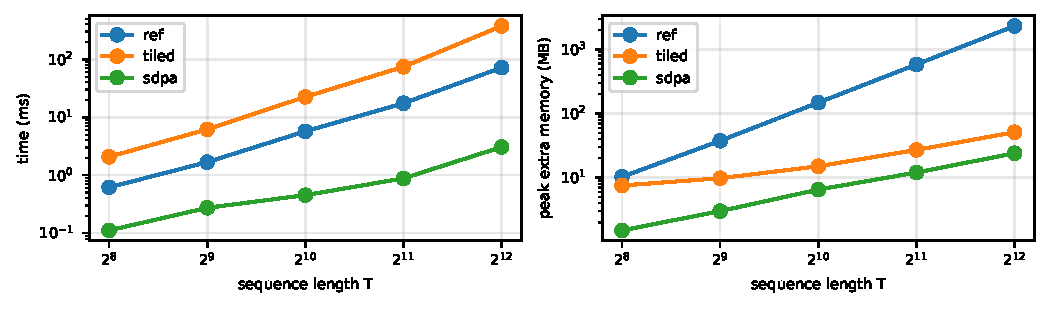
\includegraphics[width=\columnwidth]{fig_attn.pdf}
\caption{Attention time (left) and peak extra memory (right) versus sequence length.}
\label{fig:attn}
\end{figure}

\subsection{Speculative Decoding (Task 5)}
The draft is the fine-tuned Qwen2.5-0.5B (same tokenizer; 0.92\,GB in fp16; 12\,KiB KV cache per token), the target the fine-tuned 1.5B model; we run the 40 test prompts $\{0,5,10,\dots\}$ with the natural stop token. Table~\ref{tab:spec} and Fig.~\ref{fig:spec} give the results. Acceptance is high (94\% for $K{=}2$, 86--87\% for $K{\ge}4$) because the answer is a short, nearly deterministic JSON string, and a round emits 2.8--5.5 tokens. In fp16, 38 of 40 outputs are token-identical to target-only greedy decoding for every $K$; the two mismatches (prompts 5 and 90, at generated positions 4 and 11) are the same for all $K$. In fp32 the decoder is identical on all 20 prompts tested, so the two fp16 mismatches come from the target's $(K{+}1)$-token verification pass having different rounding from the one-token pass, which flips a near-tie; they do not indicate a logic error. Hugging Face assisted generation (with the penalty disabled) agrees with our cached greedy output on 18 of 20 prompts, the same kind of fp16 differences.

Despite the high acceptance, speculative decoding is \emph{slower} than plain cached decoding: $0.90\times$, $0.82\times$ and $0.81\times$ for $K{=}2,4,6$. The measurements explain why. In an isolated, synchronised measurement at a 512-token context the 0.5B draft takes 43.07\,ms per decoded token and the 1.5B target 43.03\,ms (cost ratio $c{=}1.00$; the pipelined decode loop of Table~\ref{tab:cache} is somewhat faster, about 35\,ms per token), because both are limited by launch overhead of 24 vs.\ 28 layers rather than by arithmetic; a 5-token verification pass costs 39\,ms, as much as a single-token step. A round with $K$ drafts therefore costs about $K\cdot 43+39$\,ms and emits $\bar n$ tokens, giving $\approx\bar n/(K+0.9)$ times the cached speed: $2.80/2.9{=}0.97$ for $K{=}2$ and $4.19/4.9{=}0.86$ for $K{=}4$, close to the measured values (the remainder is synchronisation of host-side comparisons). A speedup would require a cheaper draft step, e.g.\ via CUDA graphs or a fused decoder (for $c{=}0.3$, $K{=}4$ the same model predicts $4.19/(4\cdot0.3+0.9)\approx2.0\times$; this projection is not measured). Peak extra memory for speculative decoding is only 26--27\,MB beyond the resident weights of both models (about 4.0\,GB).

\begin{table}[t]
\caption{Greedy speculative decoding on 40 real test prompts (fp16). Latency is per prompt; speedup is cached time divided by speculative time.}
\label{tab:spec}
\centering\scriptsize
\begin{tabular}{rcccccc}\toprule K & Token-identical & Accept. & Tok/round & Spec s & Cached s & Speedup\\\midrule
2 & 38/40 & 0.94 & 2.80 & 0.650 & 0.584 & 0.90$\times$\\
4 & 38/40 & 0.87 & 4.19 & 0.686 & 0.560 & 0.82$\times$\\
6 & 38/40 & 0.86 & 5.53 & 0.697 & 0.562 & 0.81$\times$\\
\bottomrule\end{tabular}
\end{table}

\begin{figure}[t]
\centering
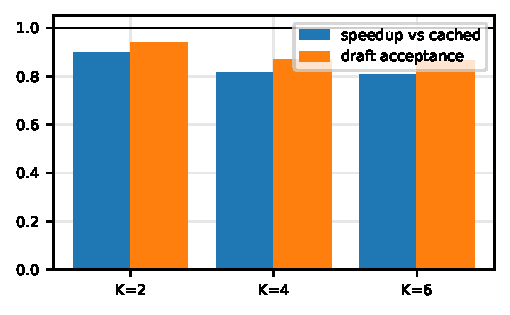
\includegraphics[width=0.8\columnwidth]{fig_spec.pdf}
\caption{Speculative decoding: speedup relative to cached decoding (values below 1 are slowdowns) and draft acceptance rate for each $K$.}
\label{fig:spec}
\end{figure}

\subsection{Application (Task 6)}
The browser application (FastAPI back end, single-page front end, no notebook needed) loads both models once at start-up, shows loading progress and the device, and offers five tabs. \emph{Screening} accepts a pasted note and any number of criteria, runs the chosen decoder, and for each criterion shows the label, the cited sentences with their text, an evidence-based explanation, flags (\emph{unsupported}, invalid output, non-existent sentence IDs), timing and, for speculative mode, the draft acceptance; it aggregates the labels with rules R1--R4 and exports an HTML or JSON report containing provenance (models, adapter checksum, mode, timestamp) and the research-prototype disclaimer. \emph{Inference lab} runs the same criteria through the three decoders, reporting time, tokens/s, peak GPU memory, draft acceptance and a token-equality check. \emph{Attention lab} runs the reference, tiled and SDPA kernels on random tensors of the requested size and reports time, memory and error against fp64. \emph{Experiments} renders the saved result tables. Invalid inputs (empty or oversize note, malformed criteria, unknown mode, out-of-range attention parameters) return readable error messages and leave the server running. We exercised the HTTP interface with a synthetic note and five criteria in the cached and speculative modes (identical labels and evidence), the comparison and attention endpoints (all three decoders token-identical), and each error case. On the synthetic case the application flagged two exclusion answers (``heart failure'', ``anticoagulant therapy'') as unsupported because the model labelled them \emph{not excluded} without citing evidence, even though the note states that the patient denies heart failure: an example of the exclusion weakness discussed above and of why such flags are shown to the user.


\section{Design Decisions, Rejected Options and Difficulties}
\textbf{Decisions backed by evidence.}
(1)~\emph{Target model.} We selected Qwen2.5-1.5B over the 3B, SmolLM2-1.7B and TinyLlama-1.1B alternatives based on memory requirements, licence, KV-cache size and compatibility with the draft model (Table~\ref{tab:models}). We did not fine-tune the other candidates, so this decision is based on their technical properties rather than a direct comparison of model accuracy.
(2)~\emph{LoRA instead of full fine-tuning.} We went with LoRA because it requires training only 18.5M parameters. This makes it suitable for the T4 GPU and keeps the final adapter relatively small at 74\,MB, which is also easier to host.
(3)~\emph{Class balancing.} We kept the sampling weight $n_c^{-0.5}$ instead of using the more aggressive $n_c^{-1}$. We tested both approaches, and the results showed that stronger balancing actually reduced the best validation macro-F1 from 0.481 to 0.395 and accuracy from 0.680 to 0.626. Based on this comparison, we decided to keep the original weighting.
(4)~\emph{Selection rule.} Before evaluating the test set, we decided to select the checkpoint with the best validation macro-F1. Following this rule, epoch~1 was selected, even though later epochs achieved better accuracy or evidence F1 (Fig.~\ref{fig:train}). We kept the original selection criterion rather than changing it based on the results we observed later.
(5)~\emph{Output format.} We decided to generate a small JSON object from the model and parse it afterwards. We also considered constrained decoding to ensure valid labels, but the results showed that it was not necessary. The base model produced 7 invalid outputs on the test set, while the fine-tuned model produced none.
(6)~\emph{Custom inference engine.} We implemented our own forward pass so that we could explicitly manage and understand the KV cache, attention masks and positional information. Before using it for experiments, we verified its correctness against Hugging Face. The difference between the fp32 logits was only $8.5\times10^{-5}$, giving us confidence in our implementation.

\textbf{Difficulties and how we resolved them.}
\emph{Mismatch with reference decoding.} Initially, our inference engine disagreed with Hugging Face \texttt{generate} on 6 out of 9 forced-length tests. However, when we checked the forward pass in fp32, it was correct. After further investigation, we found that the default Hugging Face configuration applies a repetition penalty of 1.1. Once we disabled this penalty, all 9 cases and all 206 test prompts matched.
\emph{Incorrect speculative decoding statistics.} Our first benchmark reported fewer than one token per round and showed a $4\times$ slowdown. Since generating fewer than one token per round did not make sense, we went back and inspected the decoding loop. We found that encountering a stop token inside an accepted block did not actually terminate generation. As a result, the loop continued until the length limit and the output was trimmed afterwards. The generated outputs were correct, but the performance measurements were not. We fixed the stopping condition and ran the benchmarks again. All reported results are from the corrected implementation.
\emph{Numerical differences in fp16.} We observed that 2 out of 40 speculative decoding outputs differed from target-only greedy decoding in fp16. Instead of simply treating these differences as numerical noise, we tested the same implementation in fp32. All 20 fp32 prompts produced identical outputs, so we reported the fp16 differences rather than ignoring them.
\emph{Infrastructure-related issues.} We also faced a few problems with the available computing environment. Free Colab limits the number of concurrent sessions per account, and our first fp32 verification run exhausted the host memory, causing the notebook to restart and terminate queued jobs. In another case, leftover GPU memory from a previously failed cell caused an out-of-memory error during training. We also encountered a compatibility issue with the \texttt{torchao} package that affected PEFT. These issues cost us additional time, but they did not change the final results. We re-ran the affected jobs to make sure the reported results came from successful runs.
\emph{Experiments not performed.} There were several additional experiments we could have explored, but did not have enough time or resources to include. These include testing an untuned 0.5B draft model, trying different LoRA ranks, extending the training duration, retrieving related criteria and running experiments with multiple random seeds. We have not made any claims about these experiments or their potential results.

\section{Limitations}
The corpus has only 53 patients, and the validation and test sets contain 8 patients each, so class-level scores for rare labels (e.g.\ \emph{not included}) rest on a handful of examples and are statistically fragile. We report one training run per configuration without confidence intervals. Evidence is predicted as sentence IDs and the system never produces free-text rationales; the displayed explanation is assembled from the cited sentences. The note sentence splitter in the application is rule based and can fail on abbreviations. All timings come from one T4 GPU in fp16 with a pure-PyTorch engine; Python launch overhead dominates small-batch decoding, so absolute speedups would differ with fused kernels or larger batches. Speculative decoding is verified only for greedy decoding. The system is a research prototype and must not be used to make enrolment decisions.

\section{Conclusion}
We built and verified a complete, open, T4-sized pipeline for criterion-level trial screening: a LoRA-tuned Qwen2.5-1.5B classifier with evidence citation, a transparent hand-written inference engine whose cache, tiled attention and speculative decoder match their references, and a browser application that makes the decisions, evidence and decoder behaviour inspectable. The measurements show where each mechanism helps and where it does not, which is the main practical lesson of the project.

\section*{Availability}
Source code, logs, split manifest and results: \url{https://github.com/MusaxKhan/trialmatch}. Fine-tuned LoRA adapters (target and draft): \url{https://github.com/MusaxKhan/trialmatch/releases/download/v1.0/adapters.zip}; \texttt{scripts/download\_adapters.py} downloads and unpacks them. The repository README gives startup instructions for the browser application and the commands that reproduce every experiment on a free Colab T4. A clean Colab runtime that cloned the repository and fetched the adapters from the release started the application successfully, and the demonstration video was recorded from that instance. Demonstration video (5--7 minutes): \url{https://github.com/MusaxKhan/trialmatch/releases/download/v1.0/TrialMatch_demo_23i-0526.mp4}.

\appendices
\section{AI Assistance and Reuse Statement}
AI-assisted tools were used during the development of the initial code and report under the author's direction. The assistant was Anthropic Claude, used through Claude Code with browser control of Google Colab. The author supervised the process, reviewed the generated work and takes responsibility for the final submission. Existing libraries and frameworks were also used for standard tasks such as tokenisation, model loading, fine-tuning and evaluation (Transformers, PEFT, PyTorch, scikit-learn, FastAPI).

During the development process, we also referred to a few publicly available projects to understand different implementation approaches and design choices: the public repositories TrialMatch-KV, genai-assignment-2 and GENAI-A2-. Some of their general ideas helped guide our implementation (the Qwen2.5-1.5B/0.5B target/draft pair, class-balanced sampling, majority and first-sentence baselines, rule-based aggregation of criterion labels, and a live decoder-comparison tab), but the actual code was developed and adapted within our own codebase. All model adapters were trained by us using the prescribed dataset split, and no pre-trained weights or trained adapters from those repositories were used. Similarly, external model-generated outputs (the GPT-4 predictions in the dataset) were not used as training inputs or for evaluation.

The author takes full responsibility for the submitted work and is prepared to explain, run or modify any part of the implementation during the defense.

\begin{thebibliography}{00}
\bibitem{trialgpt} Q.~Jin \emph{et al.}, ``Matching patients to clinical trials with large language models,'' \emph{Nature Communications}, vol.~15, art.~9074, 2024.
\bibitem{qwen25} A.~Yang \emph{et al.}, ``Qwen2.5 technical report,'' arXiv:2412.15115, 2024.
\bibitem{lora} E.~J. Hu \emph{et al.}, ``LoRA: Low-rank adaptation of large language models,'' in \emph{Proc. ICLR}, 2022.
\bibitem{qlora} T.~Dettmers \emph{et al.}, ``QLoRA: Efficient finetuning of quantized LLMs,'' in \emph{Proc. NeurIPS}, 2023.
\bibitem{transformer} A.~Vaswani \emph{et al.}, ``Attention is all you need,'' in \emph{Proc. NeurIPS}, 2017.
\bibitem{gqa} J.~Ainslie \emph{et al.}, ``GQA: Training generalized multi-query transformer models from multi-head checkpoints,'' in \emph{Proc. EMNLP}, 2023.
\bibitem{rope} J.~Su \emph{et al.}, ``RoFormer: Enhanced transformer with rotary position embedding,'' \emph{Neurocomputing}, vol.~568, 2024.
\bibitem{online} M.~Milakov and N.~Gimelshein, ``Online normalizer calculation for softmax,'' arXiv:1805.02867, 2018.
\bibitem{flash} T.~Dao \emph{et al.}, ``FlashAttention: Fast and memory-efficient exact attention with IO-awareness,'' in \emph{Proc. NeurIPS}, 2022.
\bibitem{pope} R.~Pope \emph{et al.}, ``Efficiently scaling transformer inference,'' in \emph{Proc. MLSys}, 2023.
\bibitem{vllm} W.~Kwon \emph{et al.}, ``Efficient memory management for large language model serving with PagedAttention,'' in \emph{Proc. SOSP}, 2023.
\bibitem{medusa} T.~Cai \emph{et al.}, ``Medusa: Simple LLM inference acceleration framework with multiple decoding heads,'' in \emph{Proc. ICML}, 2024.
\bibitem{eagle} Y.~Li \emph{et al.}, ``EAGLE: Speculative sampling requires rethinking feature uncertainty,'' in \emph{Proc. ICML}, 2024.
\bibitem{specdec} Y.~Leviathan, M.~Kalman, and Y.~Matias, ``Fast inference from transformers via speculative decoding,'' in \emph{Proc. ICML}, 2023.
\bibitem{specsamp} C.~Chen \emph{et al.}, ``Accelerating large language model decoding with speculative sampling,'' arXiv:2302.01318, 2023.
\end{thebibliography}

\end{document}
